% This is "sig-alternate.tex" V2.0 May 2012
% This file should be compiled with V2.5 of "sig-alternate.cls" May 2012
%
% This example file demonstrates the use of the 'sig-alternate.cls'
% V2.5 LaTeX2e document class file. It is for those submitting
% articles to ACM Conference Proceedings WHO DO NOT WISH TO
% STRICTLY ADHERE TO THE SIGS (PUBS-BOARD-ENDORSED) STYLE.
% The 'sig-alternate.cls' file will produce a similar-looking,
% albeit, 'tighter' paper resulting in, invariably, fewer pages.
%
% ----------------------------------------------------------------------------------------------------------------
% This .tex file (and associated .cls V2.5) produces:
%       1) The Permission Statement
%       2) The Conference (location) Info information
%       3) The Copyright Line with ACM data
%       4) NO page numbers
%
% as against the acm_proc_article-sp.cls file which
% DOES NOT produce 1) thru' 3) above.
%
% Using 'sig-alternate.cls' you have control, however, from within
% the source .tex file, over both the CopyrightYear
% (defaulted to 200X) and the ACM Copyright Data
% (defaulted to X-XXXXX-XX-X/XX/XX).
% e.g.
% \CopyrightYear{2007} will cause 2007 to appear in the copyright line.
% \crdata{0-12345-67-8/90/12} will cause 0-12345-67-8/90/12 to appear in the copyright line.
%
% ---------------------------------------------------------------------------------------------------------------
% This .tex source is an example which *does* use
% the .bib file (from which the .bbl file % is produced).
% REMEMBER HOWEVER: After having produced the .bbl file,
% and prior to final submission, you *NEED* to 'insert'
% your .bbl file into your source .tex file so as to provide
% ONE 'self-contained' source file.
%
% ================= IF YOU HAVE QUESTIONS =======================
% Questions regarding the SIGS styles, SIGS policies and
% procedures, Conferences etc. should be sent to
% Adrienne Griscti (griscti@acm.org)
%
% Technical questions _only_ to
% Gerald Murray (murray@hq.acm.org)
% ===============================================================
%
% For tracking purposes - this is V2.0 - May 2012

\documentclass{sig-alternate}
\usepackage{adjustbox}
\usepackage{graphicx}
\usepackage{multirow}
\usepackage{pdflscape}
\usepackage{subcaption}
\usepackage{url}


\begin{document}
%
% --- Author Metadata here ---
%\conferenceinfo{WOODSTOCK}{'97 El Paso, Texas USA}
%\CopyrightYear{2007} % Allows default copyright year (20XX) to be over-ridden - IF NEED BE.
%\crdata{0-12345-67-8/90/01}  % Allows default copyright data (0-89791-88-6/97/05) to be over-ridden - IF NEED BE.
% --- End of Author Metadata ---

\title{Analyzing e-cigarette sentiment on Twitter}
%
% You need the command \numberofauthors to handle the 'placement
% and alignment' of the authors beneath the title.
%
% For aesthetic reasons, we recommend 'three authors at a time'
% i.e. three 'name/affiliation blocks' be placed beneath the title.
%
% NOTE: You are NOT restricted in how many 'rows' of
% "name/affiliations" may appear. We just ask that you restrict
% the number of 'columns' to three.
%
% Because of the available 'opening page real-estate'
% we ask you to refrain from putting more than six authors
% (two rows with three columns) beneath the article title.
% More than six makes the first-page appear very cluttered indeed.
%
% Use the \alignauthor commands to handle the names
% and affiliations for an 'aesthetic maximum' of six authors.
% Add names, affiliations, addresses for
% the seventh etc. author(s) as the argument for the
% \additionalauthors command.
% These 'additional authors' will be output/set for you
% without further effort on your part as the last section in
% the body of your article BEFORE References or any Appendices.

\numberofauthors{1} %  in this sample file, there are a *total*
% of EIGHT authors. SIX appear on the 'first-page' (for formatting
% reasons) and the remaining two appear in the \additionalauthors section.
%
\author{
% You can go ahead and credit any number of authors here,
% e.g. one 'row of three' or two rows (consisting of one row of three
% and a second row of one, two or three).
%
% The command \alignauthor (no curly braces needed) should
% precede each author name, affiliation/snail-mail address and
% e-mail address. Additionally, tag each line of
% affiliation/address with \affaddr, and tag the
% e-mail address with \email.
%
% 1st. author
\alignauthor
Elaine Cristina Resende and Aron Culotta\\
       \affaddr{Department of Computer Science}\\
       \affaddr{Illinois Institute of Technology}\\
       \affaddr{Chicago, IL}\\
       \email{eresende@hawk.iit.edu, culotta@cs.iit.edu}
}
% There's nothing stopping you putting the seventh, eighth, etc.
% author on the opening page (as the 'third row') but we ask,
% for aesthetic reasons that you place these 'additional authors'
% in the \additional authors block, viz.
\additionalauthors{Additional authors: John Smith (The Th{\o}rv{\"a}ld Group,
email: {\texttt{jsmith@affiliation.org}}) and Julius P.~Kumquat
(The Kumquat Consortium, email: {\texttt{jpkumquat@consortium.net}}).}
\date{30 July 1999}
% Just remember to make sure that the TOTAL number of authors
% is the number that will appear on the first page PLUS the
% number that will appear in the \additionalauthors section.

\maketitle
\begin{abstract}
Social media platforms, such as Twitter plays a big role in the society nowadays and they have become an important source for public health surveillance and others applications. Electronic cigarette is an outstanding topic in the health area nowadays, and one important question that arises is to know how people are dealing with this new idea of "smoking free", in other words, how they are concerned about e-cigs? In order to answer questions like that we need to know what people are saying about e-cigs, if it is positive or negative and how this sentiment changes over the time. In this project, we have been working with Twitter data and we have tried to find out the sentiment of the users related to electronic cigarettes. Through our analysis we have noticed interesting facts that can contribute to the marketing and health campaigns, and also that most of sentiment is negative (marketing or criticism). 
\end{abstract}

% A category with the (minimum) three required fields
\category{I.5.4}{Pattern Recognition}{Applications--Text processing}
\category{H.4}{Information Systems Applications}{Miscellaneous}
%A category including the fourth, optional field follows...
%\category{D.2.8}{Software Engineering}{Metrics}[complexity measures, performance measures]

\keywords{Web mining, social media, public health}

\section{Introduction}

Electronic cigarettes (e-cigs) provide a nicotine-coitaining aerosol with different flavors, glycol and other ingredients, that users smoke by heating up a solution \cite{grana2014cigarettes}. There are some researches being done to confirm how harmful e-cigs can be, such as \cite{sussan2015exposure,pauly2007tobacco}, but e-cigs have not been still well studied and the effects of long-term use is not known yet \cite{bhatnagar2014electronic}.
King et al.\cite{king2013awareness} state that electronic cigarettes use is increasing a lot among adults, and \cite{centers2013notes,ecig2015triples} also describes that the use among middle school students increased, and for high school students tripled in 2014.
In this project we have been working with twitter data which was collected during a year period, from October 2012 through September 2013, looking for mentions and for people talking about e-cigs. The main goal of this project is analyze what Twitter users are talking about this subject, and try to get the sentiment of the users towards e-cigs, in order to find out how people are receiving the use of e-cigs and also to check the type of customers who are buying them. 

\section{Prior work}

\cite{myslin2013using} collected twitter data and analysed tobacco-related posts from November 2011 through July 2012, right before our data collection which was from October 2012 through September 2013. They used three machine learning algorithms and varied parameters, such as n-grams and the number of features used. Their final data set is composed of 7362 tweets and our data set is composed of more than 900k tweets. They were manually classified and each one of them was assigned to several categories (genre, theme and sentiment). The authors found that those tweets are usually more positive (41\%/30\% positive/negative ratio) towards tobacco, specially tweets related to hooka and e-cigarettes. Fist-hand personal experience is more correlated with positive sentiment and opinion correlates more strongly with negative sentiment. They also found that social factors influence in the sentiment toward tobacco. Young users and social relationships are keys that emerge with positive sentiment, what tells that positive sentiment has a interaction between hooka and e-cigarettes, younger users and positive social experiences. 

This paper focused on analysing tobacco-related tweets, positive and negative sentiment, but it does not report possible age and gender of the users. So, our study fills this gap by inferring gender and age of Twitter users in order to address the problem to monitor closely certain ages and also to drive public health campaigns to the right public.



\section{Methods}
\subsection{Data Collection}
\label{sec:data}
Tweets were collected through keywords about electronic cigarettes (e-cigarette,ecigarette, e-cig, or ecig). Same data collection process was done in this study as in the work \cite{huang2014cross}. A Support Vector Machine (SVM) algorithm was used to classify tweets in two classes commercial, which linked to commercial websites, branded promotional messages or spammer accounts, and non-commercial, which showed individual opinions and experiences. As result, 992,633 tweets were classified as organic (non-commercial), and all the collection add up to 4,639,885.

Aiming to analyze the sentiment of users we need to work just with organic tweets, so we have selected just organic tweets which represent (21.39\%) of the data. Figure \ref{figura:total} shows the number of tweets (y axis) by month (x axis). The green line refers to organic tweets and blue line to all tweets. We can see that there is a big spike in March and also an increase in the months of May and September.

\begin{figure}[t]
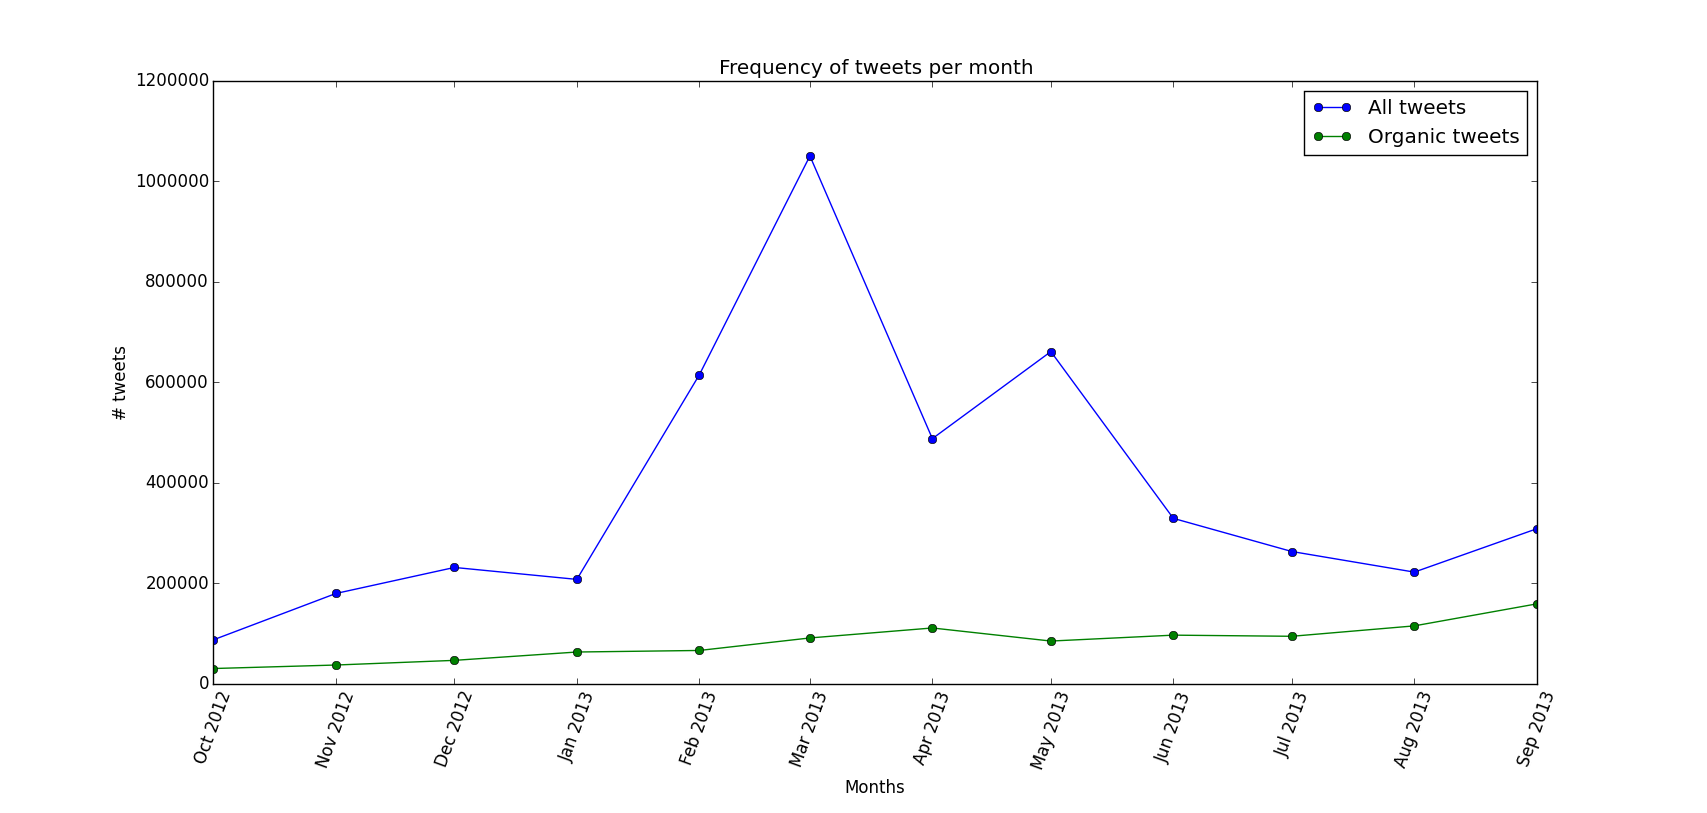
\includegraphics[width=\columnwidth]{111.png}
\caption{Number of Tweets by month}
\centering
\label{figura:total}
\end{figure}

A random sample of 2000 collected tweets, from the set of organic tweets, were manually labelled as positive, negative and neutral. Each tweet was put in one class according to the following:
\begin{itemize}
\item  tweets from merchandising companies, news about electronic cigarettes, and tweets belonging to other languages were classified as neutral class, they did not express any sentiment; 
\item  tweets from users who expressed buying or use desire, or from users who tweeted about their e-cigars were considered positive class; 
\item  and tweets from users who were complaining (or citing) about other people vaping were labelled as negative. 
\end{itemize}

Table \ref{tab:labelsample} describes some examples of our training data with tweets, their classes and also the distribution of each class. We can see that 52.45\% of the tweets were labeled as neutral, 13.75\% as negative and 33.80\% as positive. 

\begin{table*}[t]
\centering
\caption{Training Data Summary}
\label{tab:labelsample}
%\begin{adjustbox}{width=1.1\textwidth}
\begin{tabular}{|l|l|p{9cm}|}
\hline
{\bf Class}                     & {\bf \#Tweets}        & {\bf Tweet Sample}                                                                                                                       \\ \hline
\multirow{2}{*}{{\bf Positive}} & \multirow{2}{*}{676}  & I bought,a Ecig today                                                                                                                    \\ \cline{3-3} 
                                &                       & @MikeeeDeeeLeon,Nice I tried to smoke electronic cigarette last Saturday, it was my first,time.                                          \\ \hline
\multirow{2}{*}{{\bf Negative}} & \multirow{2}{*}{275}  & This kid,was hitting an e-cig during class. I look over and smokes coming out his,nose.                                                  \\ \cline{3-3} 
                                &                       & e-cigs,are bad, mmkay? {[}URL{]}                                                                                                         \\ \hline
\multirow{2}{*}{{\bf Neutral}}  & \multirow{2}{*}{1049} & \#vapor,\#smoking,\#vaping - Vapor Joes - Daily,Vaping Deals: Boge ViVi Nova - \$6.99 Free Shipping {[}URL{]},- \#ecig \#VapeDeal        \\ \cline{3-3} 
                                &                       & @SenKClark,Stop \#H3639 by @jeffrey\_sanchez , Millions have quit smoking with the \#Ecig.,\#H3639 promotes \#cigarettes and \#cancer !! \\ \hline
\end{tabular}
%\end{adjustbox}
\end{table*}

 
For this analysis we have joint negative and neutral tweets because we are more interested in the positive, in other words, telling that you use e-cigs is more important then just criticism or marketing campaigns. So, at this point we have 676 (33.8\%) tweets classified as positive and 1324 (66.2\%) as negative. The coded set of tweets was used to train a machine learning classifier using Logistic Regression algorithm, and the built model was applied to the full set of organic tweets.


\subsection{Classification}

A Logistic Regression (LG) classifier was built, trained it with coded tweets, and tested it with the organic set. Section \ref{sec:train} and \ref{sec:test} are going to show how the methodology of training and testing we followed.

\subsubsection{Training}
\label{sec:train}

A Logistic Regression classifier was used in Python language, which is responsible to predict the labels of all organic tweets; the set of labelled tweets were used as our training set. In order to have a better accuracy for the classifier, we used a grid search to check the best values for "Penalty" and "C", which are parameters of LG. Running the grid search we found out that Penalty = L2 and C = 2.6 is the best configuration for our LG model. Figure \ref{figura:para} shows the accuracy versus C parameter, and we can see that the accuracy is higher when C is equal to 2.6.

%\begin{figure}[t]
%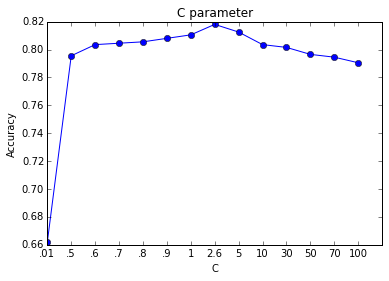
\includegraphics[width=\columnwidth]{C_parameter.png}
%\centering
%\caption{C Parameter}
%\label{figura:para}
%\end{figure}

Our best classifier configuration has the accuracy of 81.8\%. The confusion matrix of the model is shown in the Figure \ref{figura:matrix}, and Table \ref{tab:measure} shows precision, recall and F-score values for both classes. As we can notice the percentage of retrieved tweets that are relevant is 90\% what is seen as a good value for our assignment.

\begin{table}[t]
\caption{Cross-validation classification accuracy \label{tab:measure}}
\centering
\begin{tabular}{|r|c|c|c|c|}
\hline
 & {\bf Prec} & {\bf Rec} & {\bf F1} & {\bf N}\\
\hline
{\bf negative} & 0.84 & 0.83 & 0.84 & 1296\\
{\bf positive} & 0.70 & 0.72 & 0.71 & 704\\
\hline
{\bf avg} & 0.79 & 0.79 & 0.79 & 2000\\
\hline
\end{tabular}
\end{table}

%\begin{tabular}{ | l | l | l | }
%\hline
%\textbf{Measure} & \textbf{Negative Class} & \textbf{Positive Class}\\
%\hline
%Precision & 0.89745403 & 0.90614334\\
%\hline
%Recall & 0.95845921 & 0.78550296 \\
%\hline
%F-score & 0.92695398 & 0.84152139\\
%\hline
%\end{tabular}
%\label{tab:measure}
%\end{table}

\begin{figure}[t]
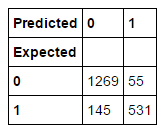
\includegraphics[width=\columnwidth]{matrix.png}
\centering
\caption{Confusion Matrix}
\label{figura:matrix}
\end{figure}

\subsubsection{Testing}
\label{sec:test}
Our testing set is defined as all organic tweets (900k tweets). The LG classifier was applied to them, as result we had 27\% classified as positive and 73\% as negative. What is comparable to our manual labeling which was 33.8\% positive and 66.2\% negative. 

In order to check the quality of our LG model, 200 tweets were randomly selected and labeled. LG model was again applied to this same new set of tweets. The labels were used as true labels and the predicted labels (output from LG model) were compared to the true labels to get the accuracy. As result, the model had 79\% of accuracy, so we conclude that our model is good for predicting the sentiment of tweets for this problem.

The top and bottom words of the classes are shown in the Table \ref{tab:coef}. Top coefficients refer to negative class and bottom coefficients show words related to positive class. Through Table \ref{tab:coef} we can see that LG model learned pretty well because words in the Top Coefficients, such as \textsc{this\_is\_a\_url}, \textsc{retail} and \textsc{stores} are related to marketing tweets, also \textsc{he}, \textsc{you}, \textsc{people} and \textsc{she} refer to other people, what represents tweets criticizing people who use e-cigs, thus being negative class. The bottom coefficients \textsc{my}, \textsc{i}, \textsc{vaping}, \textsc{vape} and \textsc{buy} refer to users who tweet about getting or using e-cigs.


\begin{table*}[t]
\centering
\caption{Top Coefficients of Classifier}
\label{tab:coef}
\begin{tabular}{|r|p{14cm}| }
\hline
{\bf negative} & you, smoking, smoking an, he, fuck, people, smokes, an, faggot, are, class, smoke, stupid, in, look, shit, her, pussy, sorry, one\\
\hline
{\bf neutral} & URL, e-cigarettes, de, la, 99, retail, URL retail, ni, e-cigarette, markten, store, by, cigarette, of, dallas, smokers, 9999, @vaper\_trail, electronic, may\\
\hline
{\bf positive} & my, i, vaping, \#vaping, \#ecig, my ecig, me, we, \#vape, got, e-cig, my e-cig, \#euecigban, my e, vape, i'm, good, this, i need, to black\\
\hline

\end{tabular}
\end{table*}


\section{Analysis of the sentiment during a year (Oct/2012-Sep/2013)}

We analyzed the amount of tweets by month according to their sentiment (negative or positive) toward e-cigs. In the Figure \ref{figura:all_org} we have considered all organic tweets. In the Figures \ref{figura:oneTweet} and \ref{figura:no_rt} it is considered just users who tweeted once. Figure \ref{figura:one} one tweet per user is considered, and in the Figure \ref{figura:no_rt} does not consider re-tweets.

\begin{figure}[t]
  \centering
  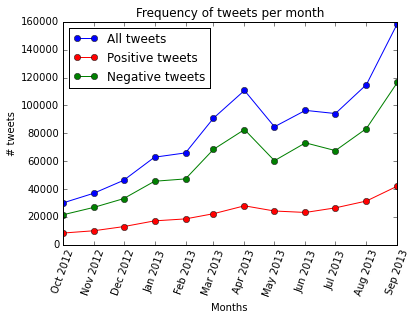
\includegraphics[width=\columnwidth]{download(1).png}
  \caption{All tweets, 1}
  \label{figura:all_org}
\end{figure}

\begin{figure*}
\begin{subfigure}{\columnwidth}
  %\centering
  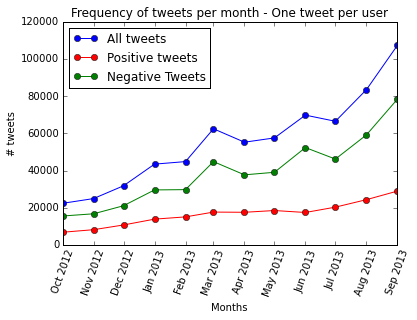
\includegraphics[width=\columnwidth]{one_per_user.png}
  \caption{All tweets}
  \label{figura:one}
\end{subfigure}%
\begin{subfigure}{\columnwidth}
  \centering
  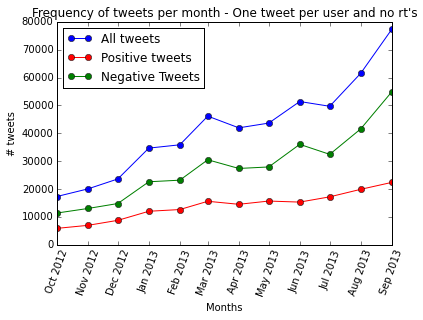
\includegraphics[width=\columnwidth]{no_rts.png}
  \caption{No re-tweets}
  \label{figura:no_rt}
\end{subfigure}%
\caption{One tweet per user}
\end{figure*}


\begin{figure*}
\begin{subfigure}{\columnwidth}
  \centering
  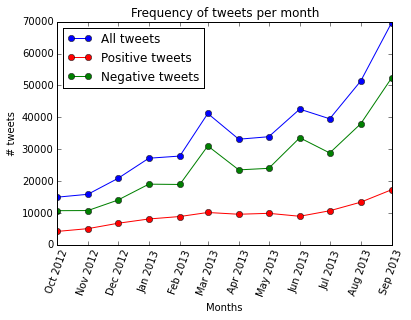
\includegraphics[width=\columnwidth]{download(2).png}
  \caption{All tweets}
  \label{figura:oneTweet}
\end{subfigure}%
\begin{subfigure}{\columnwidth}
  \centering
  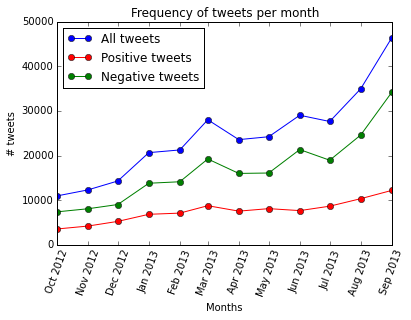
\includegraphics[width=\columnwidth]{users_tweeted_once_no_rt.png}
  \caption{No re-tweets}
  \label{figura:no_rtuser}
\end{subfigure}%
\caption{Users who tweeted once}
\end{figure*}

 In those Figures red represents positive tweets, green represents negative and blue all organic tweets. Figure \ref{figura:all_org} shows spikes in April, June and September for all sentiment lines, but Figures \ref{figura:one} and \ref{figura:oneTweet} have moved the first left spike from April to March, what tell us that the number of users was higher in March than April. Figure \ref{figura:oneTweet} and Figure \ref{figura:no_rtuser} have similar shape (same for 
Figures \ref{figura:one} and \ref{figura:no_rt}), they differ just in the number of tweets in the y axis. 

Aiming to try to find out why we have those spikes we analyzed n-grams, which are a sequence of words in the tweet, and also the 10 top words for each month during the year, shown in the Table \ref{tab:topwords}. We can see that the words in the table are very correlated with the tweets posted in the respective month. For example, November has the word \textsc{thanksgiving}, \textsc{christmas} appears in December, \textsc{valentine} in February, and so on. These words can help us to understand the spikes, and what are the main topics for positive and negative tweets. Some of the spikes are due to some events that occurred during those months. Besides the significance of each word, the Table \ref{tab:topwords} also shows the percentage of tweets that each word is present, what can describe the importance of them to the entire data. Following we have a brief analysis description of the spikes shown in the graphs. \\

\textbf{March}

Analysing Figure \ref{figura:oneTweet} which shows one tweet per user, March has 44788 negative and 17656 positive tweets. If we look in the Table \ref{tab:topwords}, the month of March shows the word \textsc{onew}, what refers to a Korean singer vaping. A lot of Twitter users tweeted about him, and most of tweets were negative. We also have the words \textsc{vatican} and \textsc{pope} which represent the month of the choice of the pope, and these are also classified most negative.\textsc{vaperware} is a store and most of the tweets are classified as negative. \textsc{swsw} is a music, film and interactive festival happening in March and most tweets are negative classified. 300 tweets were saying: \textsc{BlackFriday \#BlackFriday  is too good for me because i used electronic cigarette which  i missed a lot} and they were classified as positive tweets.

This month had about 16.5\% of users who posted positively according to Figure \ref{figura:sent}. \\
    
\textbf{April}

 
Considering just positive tweets from Figure \ref{figura:one} and going through the n-grams of the month of April we found in total 17548 tweets. After analyzing the n-grams, we took a further look in those tweets and we found more than 600 re-tweets of: \textsc{" @SimonCowell: I have cut down smoking. A lot. Using electric cigarettes to help. Are they bad for you?"} and they were labeled as positive.

According to Figures \ref{figura:sent} and \ref{figura:sent2}, April was the month which people talked less in positive way toward e-cigs. In the Table \ref{tab:topwords}, we can see that is because some senators in US made regulations to restrict the sale of e-cigars \footnote{http://www.enewspf.com/latest-news/health-and-fitness/42182-senators-call-on-fda-to-restrict-the-sale-distribution-and-marketing-of-e-cigarettes.html}, and also about Courtney TV commercial.\footnote{http://www.huffingtonpost.com/2013/04/03/courtney-love-njoy\_n\_3006660.html?ncid=edlinkusaolp00000003}

Some other words from Table \ref{tab:topwords} are described below and most of the tweets containing them were classified as negative, what contributed for negativeness in this month.

\textsc{\#\textbf{welcometomyschoolwhere} people smoke electronic cigs during class}

\textsc{E-cigarettes \textbf{primarily} used to quit tobacco: study http://t.co/l2G1DksNJt \#EUecigBAN}

\textsc{\textbf{Leachon}: E-cigarettes may contain carcinogens, ingredients not approved by FDA}\\


\textbf{September}

This month is the third most negative with 15\%  of positive tweets overall. 28938 tweets are positive and 78341 are negative according to Figure \ref{figura:one}.

The word \textbf{whisp} refers to \textsc{"RT \@YABOYLILB: *gets in booster seat*  *puts seatbelt on*  *puts in the newest kidzbop CD*  *takes drag of e-cig*  *lowers glasses*  *whisp"} and it was classified as positive.

\textbf{worldvapingday} is a hashtag about http://www.world-vaping-day.com/, which is the day of vaping, and most of them were negative. Two main tweets appeared in the data: 
\begin{enumerate}

\item \textsc{Thursday is \#WorldVapingDay!  Time to tell the world how \#Ecigs have changed your life!!!}. It was classified as negative.
\item \textsc{Thurs. is \#WorldVapingDay! Conservatives need to know the FDA will try to ban \#ecigs again in Oct. Stop liberals,save lives}. It was classified as positive.
\end{enumerate}

\textsc{ProperLongboard Vaping Dallas Party Gift E-juice \&amp; \textbf{Nude} Selfies http://t.co/mSKyyKfzZW} explains the appearance of the word nude, and they were negative tweets.

The word \textbf{attorneys} represents tweets saying about e-cigarette regulations. E.g.: \textsc{vegasnewsnow Attorneys general call on FDA to regulate e-cigarettes [URL] \#vegas}. Most classified as negative.

\textbf{Vapefest} occurs during September and most of tweets were negative. E.g.: \textsc{Cant wait for \#vapefest next weekend. Stoked}

\textbf{Teens} represents tweets talking about the grow of teens vaping, and they also represent negative class. E.g.: \textsc{Bakocom Study Shows More Teens Turning To Electronic Cigarettes: \#palmsprings \#[URL]}\\

\begin{figure*}[t]
\begin{subfigure}{\columnwidth}
  %\centering
  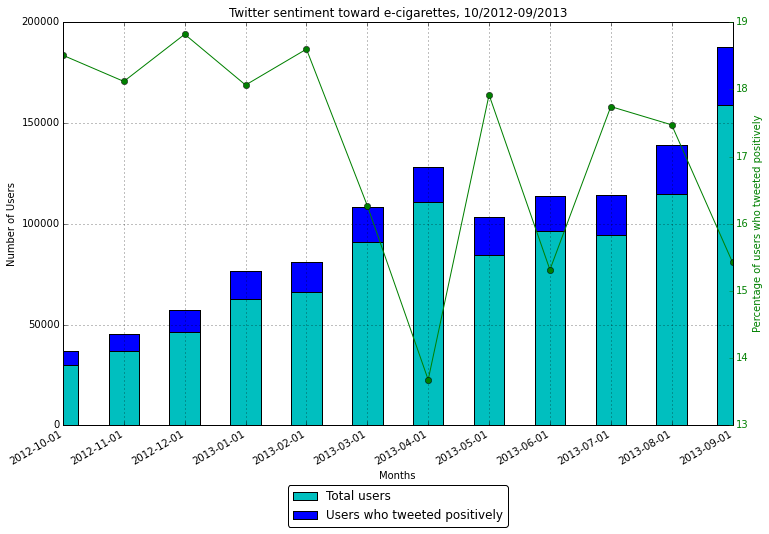
\includegraphics[width=\columnwidth]{sentiment1correct.png}
  \caption{Model using 2 classes}
  \label{figura:sent}
\end{subfigure}%
\begin{subfigure}{\columnwidth}
  %\centering
  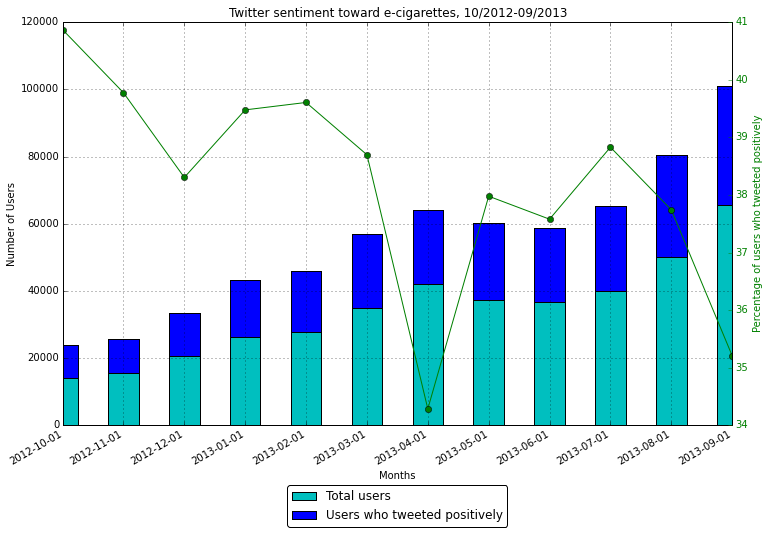
\includegraphics[width=\columnwidth]{sentiment2correct.png}
  \caption{Model using 3 classes}
  \label{figura:sent2}
\end{subfigure}%
\caption{Sentiment over the year}
\end{figure*}

Figure \ref{figura:sent} shows, in the right y axis, the percentage of positive tweets over all organic with LG model built with 2 classes (positive and negative). We can see that the percentage of positivism is higher during October, December and February, and then it goes down during March and April. May starts going up again, but for the rest of the months no one goes upper than May. The left y axis describes the number of users, and in the x axis, the bars show the number of users who are posting positively by month, from October 2012 through September 2013 in blue color, and we can notice that this number is much less than negative, what tell us that most of tweets are propaganda or criticism about someone using e-cigs. 

In order to understand more Figure \ref{figura:sent}, we have done an analysis considering the 3 classes explained in Section \ref{sec:data}. Figure \ref{figura:sent2} plots the percentage of positive tweets over the year considering positive and negative tweets from LG model using 3 classes (positive, negative and neutral). As it is expected, the percentage of positivism increases. April still is the month with less positive tweets, October is the most positive month overall.

\subsection{Gender Inference}

U.S. Census provides list of names from population. We use the 1990's census\footnote{http://www2.census.gov/topics/genealogy/} to compute the proportion of males and females for positive and negative classes. We keep 75\% of each names list, eliminate ambiguous names, at the end the total names are 226 males and 518 females. Each tweet gets then its label, if the first name of the user is present in the male list, it is labeled as male or the same for female list. Figure \ref{figura:gender} shows the distribution of genders in our data. 74\% overall tweets have their gender unknown because the users did not have their names in the census data and majority of tweets belonged to users of companies (369127 unique users are labeled as "unknown"). We can see that 28-30\% of users, independently of gender, express positive sentiment towards electronic cigarettes, but the majority express negativeness toward them.
\begin{figure}[t]
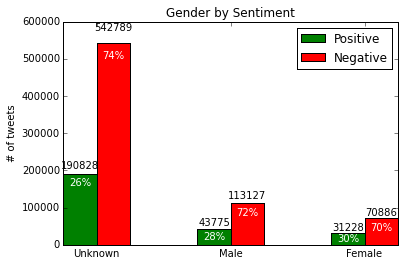
\includegraphics[width=\columnwidth]{gender.png}
\centering
\caption{ Gender distribution of Twitter users}
\label{figura:gender}
\end{figure}

\subsection{Age Inference}

In a recent study Silver and McCanc \cite{silver2014how}, showed how the age of a person can be indicated by her/his name. The Social Security Administration (SSA) provides a list of baby names\footnote{http://www.ssa.gov/oact/babynames/} who are born in each year, from 1880 to 2014. Through this list we can know gender and number of babies born with a name by year. Another resource we use to infer age is a cohort life table also provided by SSA\footnote{http://www.ssa.gov/oact/NOTES/as120/LifeTables\_Tbl\_7.html}, that give us the estimate of how many people born in a given year are still alive. 

We define the years in age brackets (under 18, 18-24, 25-34, 35-44 and 45+) and with the number of people in certain age and who are still alive we can compute the fraction of people who are still alive for each age bracket. For example, given a name we can see the fraction of people who are 18 years old, which is in the first bracket. Figure \ref{figura:age_bracket} shows an example for the name Elaine, the first column represents the brackets; "n" is the number of people who born during that period, "n\_alive" is the number of people born in that period who are still alive, and "fraction" shows the percentage of people in that bracket who are still alive. In this figure we can see that the most common age estimate for Elaine is 45+, followed by 35-44, 25-34, 18-24 and 18-.


\begin{figure}[t]
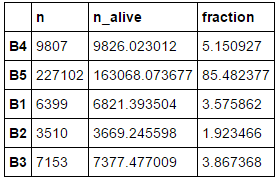
\includegraphics[width=\columnwidth]{elaine.PNG}
\centering
\caption{Age Bracket for the name Elaine}
\label{figura:age_bracket}
\end{figure}

The age inference analysis was done by month, considering both classes of our data set. The next figures show the age brackets estimates by month during the year data, plotting separately by sentiment. Figures \ref{figura:pos_45+}, \ref{figura:neg_45+}, and \ref{figura:all_45+} plot the sentiment by age for each age bracket. Figures \ref{figura:pos_45+diff}, \ref{figura:neg_45+diff}, and \ref{figura:all_45+diff} show the differences in the estimates of age. 


\begin{figure}[t]
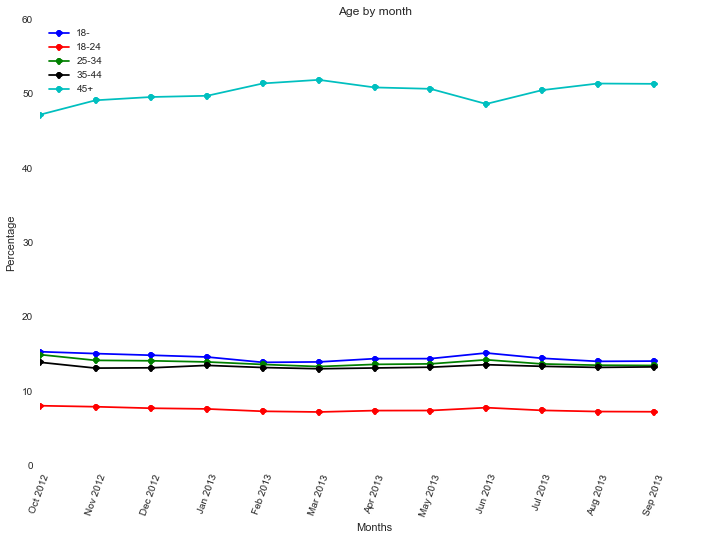
\includegraphics[width=\columnwidth]{pos_45+.png}
\centering
\caption{Age brackets estimate for positive tweets}
\label{figura:pos_45+}
\end{figure}

\begin{figure}[t]
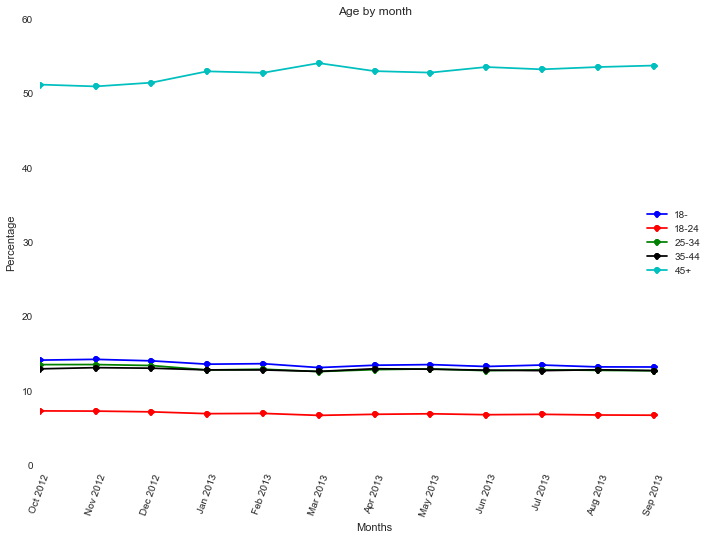
\includegraphics[width=\columnwidth]{neg_45+.png}
\centering
\caption{ Age brackets estimate for negative tweets}
\label{figura:neg_45+}
\end{figure}

\begin{figure}[t]
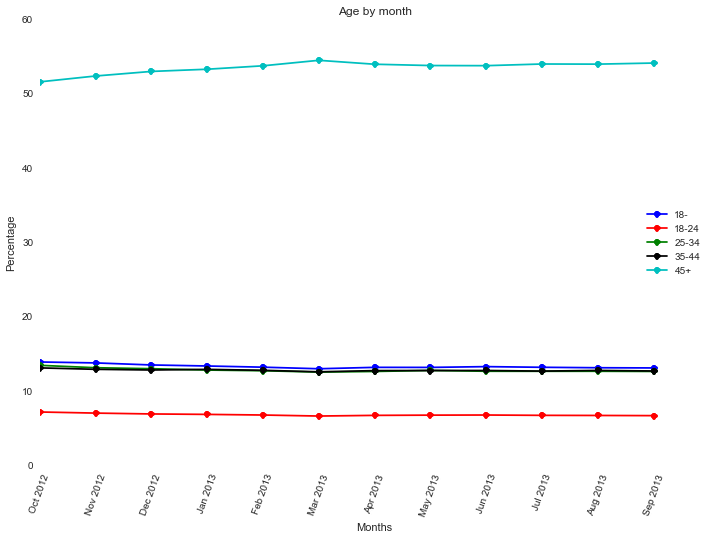
\includegraphics[width=\columnwidth]{all_45+.png}
\centering
\caption{ Age brackets estimate for all tweets}
\label{figura:all_45+}
\end{figure}


\begin{figure}[t]
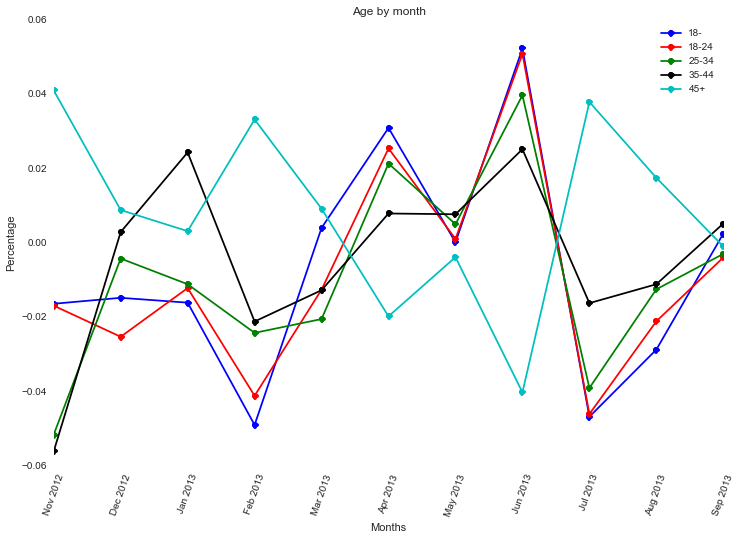
\includegraphics[width=\columnwidth]{pos_45+diff.png}
\centering
\caption{Age brackets estimate difference for positive tweets}
\label{figura:pos_45+diff}
\end{figure}

Figure \ref{figura:pos_45+diff}x

\begin{figure}[t]
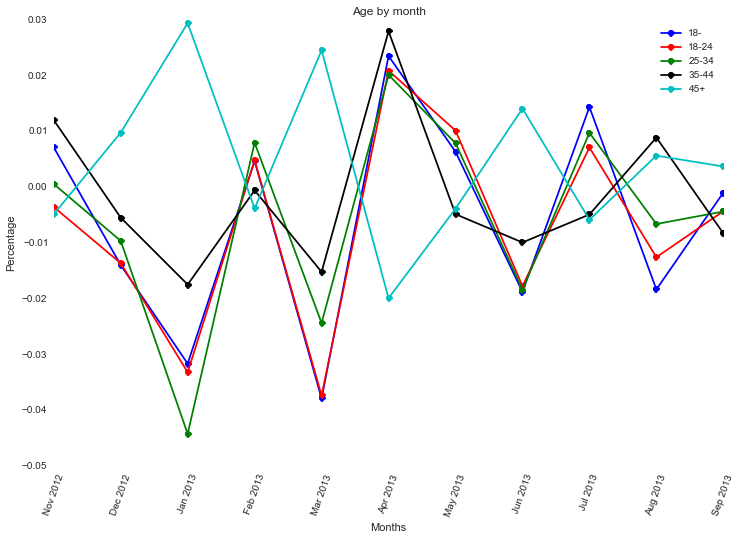
\includegraphics[width=\columnwidth]{neg_45+diff.png}
\centering
\caption{ Age brackets estimate difference for negative tweets}
\label{figura:neg_45+diff}
\end{figure}

\begin{figure}[t]
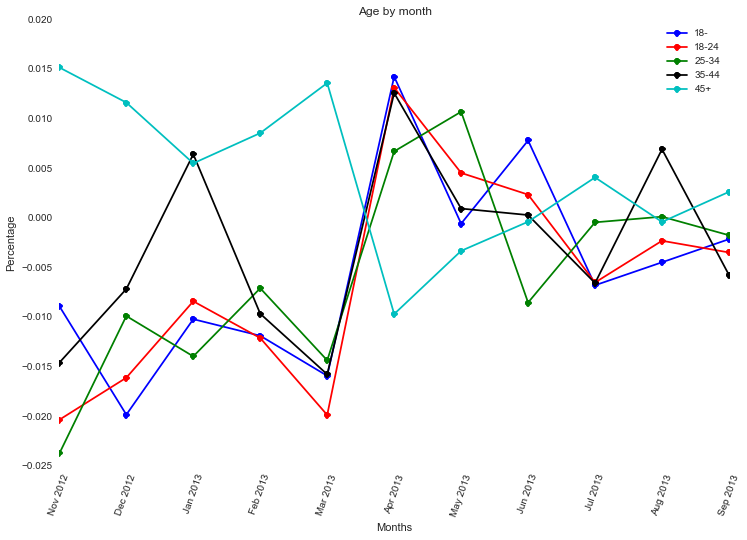
\includegraphics[width=\columnwidth]{all_45+diff.png}
\centering
\caption{ Age all brackets estimate difference for tweets}
\label{figura:all_45+diff}
\end{figure}





\begin{landscape}
\begin{table}[httb]
\caption{10 Most significant words by month}
\label{tab:topwords}
\hskip-5.0cm\begin{tabular}[httb]{ | l | l | l | l | l | l | }
\hline
	Oct & Nov & Dec & Jan & Feb & Mar \\ \hline
	dragonfly 16.81 - 1.33\% & election 10.12 - 1.70\% & mhealth 9.29 - 0.29\% & igotoaschoolwhere 8.52 - 0.20\% & whatevs 9.16 - 0.27\% & onew 12.53 - 2.98 \% \\ \hline
	ltdTHIS\_IS\_A\_URL 8.74 - 0.27\% & thanksgiving 8.61 - 0.36\% & christmas 8.26 - 2.07\% & soar 7.92 - 0.32\% & ecigs1 8.46 - 0.19\% & 03 10.78 - 2.88\% \\ \hline
	stoptober 7.89 - 1.04\% & election2012 8.17 - 0.22\% & youcantbetakenseriouslyif 7.97 - 0.12\% & mook 7.03 - 0.53\% & valentine 7.69 - 0.50\% & pope 9.96 - 4.35\% \\ \hline
	discos 6.85 - 4.22\% & sarapmagvape 7.71 - 0.45\% & ganj 7.74 - 0.28\% & embarrassment 6.85 - 0.33\% & valentines 7.13 - 0.10\% & vaporware 8.87 - 0.12\% \\ \hline
	clik 6.71 - 0.44\% & sideburn 6.81 - 0.11\% & xmas 7.11 - 0.45\% & thingsthatbotherme 6.43 - 0.21\% & queers 6.89 - 0.42 & vatican 8.15 - 1.23\% \\ \hline
	mall 6.56 - 1.70\% & pattinson 6.61 - 0.63\% & dec 7.00 - 0.29\% & 22509 5.97 - 0.07\% & superbowl 6.84 - 0.12\% & sxsw 8.10 - 0.15\% \\ \hline
	clintandrew 6.29 - 0.28\% & shishavapes 5.96 - 0.31\% & govawards 6.33 - 0.10\% & 36e 5.84 - 0.17\% & oscars 6.51 - 0.09\% & nanopartices 7.82 -0.09\% \\ \hline
	fuckingsmart 6.28 - 0.23\% & nov 5.64 - 0.21\% & itsabaddaywhen 6.09 - 0.21\% & pst 5.84 - 0.10\% & baftas 6.49 - 0.09\% & conclave 7.71 - 1.01\% \\ \hline
	dispoecig 6.25 - 0.12\% & emazin 5.60 - 0.10\% & camilla 5.91 - 2.63\% & perfects 5.81 - 0.10\% & positivity 6.11 - 0.06\% & faked 7.49 - 0.61\% \\ \hline
	ohmyvapor 6.06 - 0.12\% & rob 5.47 - 1.73\% & legalise 5.91 - 0.28\% & monumental 5.79 0.34\% & britons 6.00 - 0.12\% & quitsmoking2 7.32 - 0.09\% \\ \hline
\end{tabular}

\hskip-5.0cm \begin{tabular}{ | l | l | l | l | l | l | }
\hline
	Apr & May & Jun & Jul & Aug & Sep \\ \hline
	courtney 13.21 - 1.41\% & efags 10.50 - 0.44\% & financile 9.57 - 0.20\% & uncut 8.34 - 0.06\% & bloomberg 9.17 - 0.90\% & whisp 14.50 - 1.42\% \\ \hline
	senators 12.17  - 0.20\% & efags2 9.40 - 0.17\% & boomed 7.54 - 0.20\% & bbj 7.61 0.51\% & proudtovape 8.25 - 0.15\% & worldvapingday 9.76 - 0.66\% \\ \hline
	euecigban 11.55 - 12.86\% & uae 8.66 - 0.28\% & fathers 7.06 - 0.11\% & modeltwo 7.17 - 0.45\% & playbook 8.21 - 0.19\% & nude 9.41 - 0.85\% \\ \hline
	primarily 9.08 - 0.16\% & 1250 8.24 - 0.17\% & mhra 6.87 - 0.91\% & lirr 7.02 - 0.09\% & kv2 7.87 - 0.09\% & attorneys 9.05 - 0.67\% \\ \hline
	leachon 8.60 - 0.13\% & workshop 8.08 - 0.33\% & rachet 6.74 - 0.24\% & ankle 7.01 - 0.11\% & 08 7.61 - 0.24\% & patches 8.68 - 2.90\% \\ \hline
	welcometomyschoolwhere  7.99 - 0.11\% & subculture 6.83 - 0.13\% & fuels 6.58 - 0.17\% & dumbasses 6.57 - 0.17\% & smartcigs 7.39 - 0.05\% & lab13 8.07 - 0.08\% \\ \hline
	750 7.90 - 2.81\% & imu 6.54 - 0.56\% & blucigscoupons 6.56 - 0.03\% & manhattan 6.49 - 0.20\% & stupider 7.35 - 0.11\% & teens 7.88 - 1.40\% \\ \hline
	eue 7.79 - 0.45\% & jury 6.49 - 0.21\% & sowwy 6.48 - 0.12\% & muffler 6.09 - 0.20\% & mass 7.20 - 0.62\% & vapefest 7.61 - 0.24\% \\ \hline
	mywebcamTHIS\_IS\_A\_MENTION 7.65 - 0.23\% & interpretations 6.39 - 0.08\% & bonnaroo 6.46 - 0.08\% & agrees 5.91 - 0.13\% & musicians 6.56 - 0.16\% & duluth 7.46 - 0.14\% \\ \hline
	irs 7.57 - 0.12\% & blogengage 6.38 - 0.09\% & restrictions 6.29 - 0.86\% & pnoy 5.78 - 0.07\% & ushered 6.51 - 0.47\% & students 7.39 - 1.59\% \\ \hline
\end{tabular}
\end{table}
\end{landscape}



\section{Conclusion}

As we could notice from our analysis the over all tweets increase over the time, but negative tweets (marketing, criticism) increases more than positive tweets. Most of tweets are negative and the positive tweets don't change much over the time, they remain around 16\% and 23\%. Most of the spikes that the Figures showed are due to a particular event during its respective month. So, we are sure that TV commercials and new campaigns are relevant and they help to make changes in the data.
\bibliographystyle{abbrv}
\bibliography{report}  % sigproc.bib is the name of the Bibliography in this case
% You must have a proper ".bib" file
%  and remember to run:
% latex bibtex latex latex
% to resolve all references
%
% ACM needs 'a single self-contained file'!
%
%\balancecolumns % GM June 2007
% That's all folks!
\end{document}
